\documentclass[11pt,a4paper]{article}
\usepackage[utf8]{inputenc}
\usepackage[english]{babel}
\usepackage[left=2.5cm, right=2.5cm, top=2.5cm, bottom=2.5cm]{geometry}
\usepackage{hyperref}
\usepackage{graphicx}
\usepackage{times}
\usepackage[bottom]{footmisc}
\usepackage{listings}
\usepackage{bm}
\usepackage{amsmath}
\usepackage{algpseudocode}
\usepackage{algorithm}
\usepackage{titlesec}
\usepackage{booktabs}
\usepackage{amsmath}


\titleformat{\subsubsection}[runin]{}{}{}{}[]

\title{\textbf{Advanced Machine Learning -- Homework 1}}
\author{Anna Berger, Ashwin Sadananda Bhat (AML25)}


\begin{document}
	\maketitle
	
	In the following exercises we use the shortened notation: $ P(C = c_0) = P(c_0).$
	\section*{Exercise 1}
	
	
	\subsection*{Part a}
	
	From the Bayesian network given in the exercise we can write the joint distribution of five variables as follows:
	
	$$ P(C,D,I,G,S) = P(C) \cdot  P(D|C)\cdot  P(I|D) \cdot  P(G|D,I) \cdot  P(S|I) $$ 
	
	In order to find $P(G)$, we marginalise over all other variables:
	
	$$ P(G) = \sum_{C, D, I, S} P(C) \cdot  P(D|C)\cdot P(I|D)\cdot P(G|D,I)\cdot P(S|I) $$ 
	
	Rearranging the summations, we get the following equation which is easier to compute:
	$$ P(G) = \sum_{D, I} P(G|D,I)\cdot P(I|D) \sum_{S} P(S | I)  \sum_{C} P(C) \cdot  P(D|C) $$ 
	
	First, we compute $ \phi_1(D) =  \sum_{C} P(C) \cdot  P(D|C): $
	
	\begin{itemize}
		\item $ \phi_1(d_0) = P(d_0 | c_0) P(c_0) + P(d_0 | c_1) P(c_1) = 0.1 \cdot 0.3 + 0.7 \cdot 0.7 = 0.52 $
		\item $ \phi_1(d_1) = P(d_1 | c_0) P(c_0) + P(d_1 | c_1) P(c_1) = 0.9 \cdot 0.3 + 0.3 \cdot 0.7 = 0.48 $
	\end{itemize} 
	
	$$ \phi_1(D)  = (0.52, 0.48)$$
	
	Secondly, we will make use of the fact that  $\phi_2(I) = \sum_{S} P(S | I) = (1, 1). $
	
	Then we compute $\phi_2(D, I) = P(I|D) \cdot \phi_1(D)$
	
	\begin{itemize}
		\item $\phi_2(d_0, i_0) = P(i_0 | d_0) \cdot \phi_1(d_0) = 0.6 \cdot 0.52 = 0.312 $
		\item $\phi_2(d_0, i_1) = P(i_1 | d_0) \cdot \phi_1(d_0) = 0.4 \cdot 0.52 = 0.208 $
		\item $\phi_2(d_1, i_0) = P(i_0 | d_1) \cdot \phi_1(d_1) = 0.9 \cdot 0.48 = 0.432 $
		\item $\phi_2(d_1, i_1) = P(i_1 | d_1) \cdot \phi_1(d_1) = 0.1 \cdot 0.48 = 0.048 $
	\end{itemize}
	
	$$ \phi_2(D, I) =  \left(\begin{smallmatrix} 0.312 & 0.208 \\ \\ 0.43 2 & 0.048 \end{smallmatrix} \right) $$
	
	Finally, we are left to compute $ P(G) =  \sum_{D, I} P(G|D,I) \phi_2(D, I):$
	\begin{itemize}
		\item $P(g_0) = P(g_0 | i_0, d_0) \phi_2(i_0, d_0) + P(g_0 | i_1, d_0) \phi_2(i_1, d_0) + P(g_0 | i_0, d_1) \phi_2(i_0, d_1) + P(g_0 | i_1, d_1) \phi_2(i_1, d_1) = $
		$ = 0.3 \cdot 0.312 + 0.4 \cdot 0.208 + 0.4 \cdot 0.432 + 0.6 \cdot 0.048 = 0.3784 $ 
		\item $P(g_1) = P(g_1 | i_0, d_0) \phi_2(i_0, d_0) + P(g_1 | i_1, d_0) \phi_2(i_1, d_0) + P(g_1 | i_0, d_1) \phi_2(i_0, d_1) + P(g_1 | i_1, d_1) \phi_2(i_1, d_1) = $
		$ = 0.2 \cdot 0.312 + 0.2 \cdot 0.208 + 0.3 \cdot 0.432 + 0.3 \cdot 0.048 = 0.248 $ 
		\item $P(g_2) = P(g_2 | i_0, d_0) \phi_2(i_0, d_0) + P(g_2 | i_1, d_0) \phi_2(i_1, d_0) + P(g_2 | i_0, d_1) \phi_2(i_0, d_1) + P(g_2 | i_1, d_1) \phi_2(i_1, d_1) = $
		$ = 0.5 \cdot 0.312 + 0.4 \cdot 0.208 + 0.3 \cdot 0.432 + 0.1 \cdot 0.048 = 0.3736 $ 
	\end{itemize} 
	
	All in all, we obtain $ P(G) = (0.3784, 0.248, 0.3736)$
	\subsection*{Part b}
	
	Again we use the equation for the joint distribution from the Bayesian network given in the exercise:
	
	$$ P(C,D,I,G,S) = P(C)\cdot P(D|C)\cdot P(I|D)\cdot P(G|D,I)\cdot P(S|I) $$
	
	Then we apply the Bayes rule and marginalise out  $P(S , c_0):$
	$$  P(S|c_0) = \frac{P(S, c_0)}{P( c_0)} =  \frac{\sum_{D,I,G} P(c_0,D,I,G,S)}{P(c_0)} $$
	
	
	$$ P(S|c_0) =  \frac{\sum_{D,I,G} P(c_0)\cdot P(D|C)\cdot P(I|D)\cdot P(G|D,I)\cdot P(S|I)}{P(c_0)} $$ 
	
	$$ P(S|c_0)  = \sum_{D,I,G} P(D|C)\cdot P(I|D)\cdot P(G|D,I)\cdot P(S|I) $$
	
	Rearranging the summations, we obtain the equation handy to compute:
	$$ P(S|c_0)  = \sum_{D} P(D|C) \cdot  \sum_{I}P(I|D)\cdot P(S|I) \cdot \sum_{G}P(G|D,I)  \label{eq:1.1} $$
	
	As $ \sum_{G}P(G|D,I) = 1$, then we are left to compute:
	
	$$ P(S|c_0) = \sum_{D} P(D|C) \cdot  \sum_{I}P(I|D)\cdot P(S|I)$$
	
	First we calculate $ \phi_I(S,D) = \sum_{I}P(I|D)\cdot P(S|I)$:
	\begin{itemize}
		\item $ \phi_I(s_0, d_0) = P(i_0|d_0) \cdot  P(s_0|i_0) + P(i_1|d_0) \cdot  P(s_0|i_1) $
		$ = 0.6\cdot 0.2 + 0.4\cdot 0.7 = 0.4 $
		\item $ \phi_I(s_0, d_1) = P(i_0|d_1) \cdot  P(s_0|i_0) + P(i_1|d_1) \cdot  P(s_0|i_1) $
		$ = 0.9\cdot 0.2 + 0.1\cdot 0.7 = 0.25 $
		\item $ \phi_I(s_1, d_0) = P(i_0|d_0) \cdot  P(s_1|i_0) + P(i_1|d_0) \cdot P(s_1|i_1) $
		$ = 0.6\cdot 0.8 + 0.4\cdot 0.3 = 0.6 $
		\item $ \phi_I(s_0,d_1) = P(i_0|d_1) \cdot  P(s_0|i_0) + P(i_1|d_1) \cdot P(s_0|i_1) $
		$ = 0.9\cdot 0.8 + 0.1\cdot 0.3 = 0.75 $
	\end{itemize}
	
	$$  \phi_I(S,D) =  \left(\begin{smallmatrix} 0.4 & 0.25 \\ \\ 0.6 & 0.75 \end{smallmatrix} \right) $$
	
	Then we are left to compute $ P(S|c_0) = \sum_{D}P(D|c_0) \cdot  \phi_I(S,D) :$
	\begin{itemize}
		\item $ P(s_0|c_0) = P(d_0|c_0)\cdot \phi_I(s_0,d_0) + P(d_1|c_0)\cdot \phi_I(s_0,d_1) = 0.1\cdot 0.4 + 0.9\cdot 0.25 = 0.265 $
		\item $ P(s_1|c_0) = P(d_0|c_0)\cdot \phi_I(s_1,d_0) + P(d_1|c_0)\cdot \phi_I(s_1,d_1)  = 0.1\cdot 0.6 + 0.9\cdot 0.75  = 0.735 $
	\end{itemize}
	
	Therefore, $$ P(S | c_0) = (0.265, 0.735). $$
	
	\subsection*{Part c}
	Again we use the equation for the joint distribution from the Bayesian network given in the exercise:
	$$ P(C,D,I,G,S) = P(C)\cdot P(D|C)\cdot P(I|D)\cdot P(G|D,I)\cdot P(S|I) $$
	
	First we apply the Bayes rule to compute the conditional probability distribution:
	$$ P(D | g_2) = \frac{P(D, g_2)}{P(g_2)} $$
	
	In \textbf{Part a} we have already computed $P(g_2) = 0.3736. $
	
	We marginalise over all other variables to obtain $P(D , g_2)$ and group sums:
	
	$$ P(D, g_2) = \sum_{C,S,I}P(C,D,I, g_2,S) = \sum_{C}P(C)\cdot P(D|C)\cdot \sum_{I}P(I|D) \cdot P(g_2|D,I) \cdot \sum_{S}P(S|I)$$
	
	We make use of the fact that $ \sum_{S}P(S|I) = (1, 1)$, then we are left to compute:
	$$ P(D,g_2)  = \sum_{C}P(C)\cdot P(D|C)\cdot \sum_{I}P(I|D) \cdot P(g_2|D,I)$$
	
	
	First, we calculate $ f_C(D) = \sum_{C}P(C) \cdot P(D|C): $
	\begin{itemize}
		\item $f_C(d_0) = P(c_0) \cdot P(d_0|c_0) + P(c_1) \cdot P(d_0|c_1) = 0.3 \cdot 0.1+0.7 \cdot 0.7 = 0.52$
		\item $f_C(d_1) = P(c_0) \cdot P(d_1|c_0) + P(c_1) \cdot P(d_1|c_1) = 0.3 \cdot 0.9 + 0.7 \cdot 0.3 = 0.48$
	\end{itemize}
	
	Then we compute $f_I(D) =  \sum_{I}P(I|D)\cdot P(g_2|D,I): $
	\begin{itemize}
		\item $f_I(d_0) = P(i_0|d_0) \cdot P(g_2|d_0,i_0) + P(i_1|d_0) \cdot P(g_2|d_0,i_1) = 0.6 \cdot 0.5 + 0.4 \cdot 0.4 = 0.46$
		\item $f_I(d_1) = P(i_0|d_1) \cdot P(g_2|d_1,i_0) + P(i_1|d_1) \cdot P(g_2|d_1,i_1)  = 0.9 \cdot 0.3 + 0.1 \cdot 0.1 = 0.28$
	\end{itemize} 
	
	Having computed $f_I(D)$ and $f_C(D)$, we can now compute $P(D,g_2)$ as $$P(D,g_2) = f_I(D) \cdot f_C(D): $$
	
	\begin{itemize}
		\item $P(d_0,g_2) = f_I(d_0) \cdot f_C(d_0) = 0.46  \cdot 0.52 = 0.2392 $
		\item $P(d_1,g_2) = f_I(d_1) \cdot f_C(d_1)  = 0.28  \cdot 0.48 = 0.1344 $
	\end{itemize}
	
	Now, we can do the final computation $ P(D | g_2) = \frac{P(D, g_2)}{P(g_2)} $ :
	\begin{itemize}
		\item $P(d_0|g_2) = \frac{P(d_0,g_2)}{P(g_2)} \approx 0.64 $
		\item $P(d_1|g_2) = \frac{P(d_1,g_2)}{P(g_2)} \approx 0.36 $
	\end{itemize}
	
	Therefore, $$P(D | g_2) = (0.64, 0.36).$$
	
	\newpage
	\section*{Exercise 2}
	
	In Exercise 2 we use the factor graph from the Figure \ref{fig:fgraph_2}. Although it has cycles in it, we can use it as it doesn't create any difficulties for approach with direct marginalization. However, for Exercise 3 this graph is inapplicable: as it has a cycle and the sum-product algorithm won't work properly with it.

	\begin{figure}[H]
		\centering{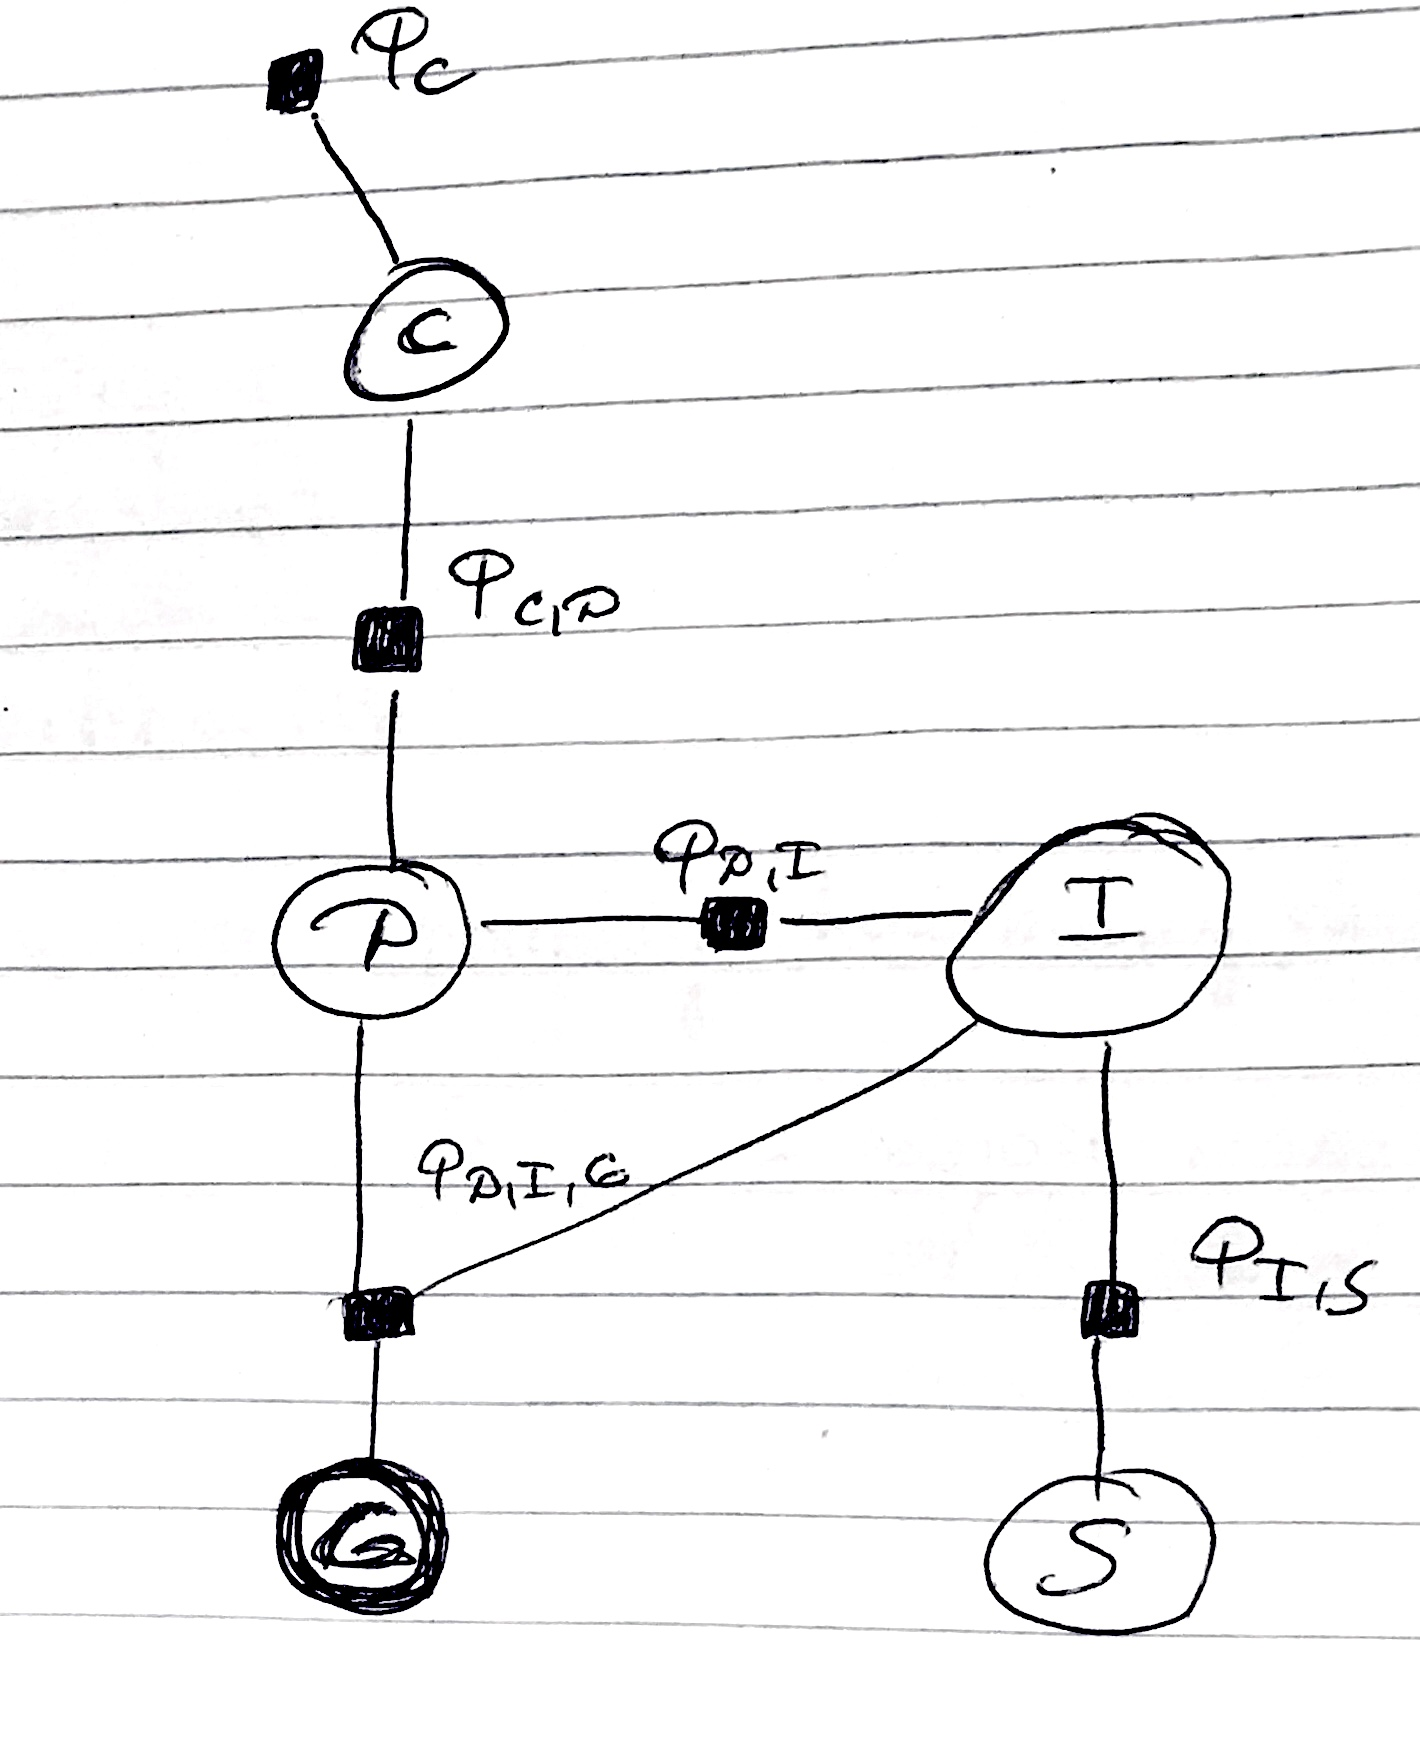
\includegraphics[height =10cm]{figures/fgraph_2.jpg}}
		\caption{Factor graph for Exercise 2}
		\label{fig:fgraph_2}
	\end{figure}
	
	\subsection*{Part a:}
	From the graph we can obtain the following equation for factors:
	$$\Phi(C,D,I,G,S) = \Phi(C) \cdot \Phi(C,D) \cdot \Phi(D,I) \cdot \Phi(D,I,G) \cdot \Phi(I,S)$$
	
	In order to compute the factor $\Phi(G)$ we marginalise over all variables except $G$:
	$$\Phi(G) = \sum_{C,D,I,S}\Phi(C,D,I,G,S)$$
	$$  \Phi(G)= \sum_{D, I} \Phi(D,I) \Phi(D,I,G)  \sum_{C}\Phi(C) \Phi(C,D) \cdot \sum_{S} \Phi(I,S)$$
	
	First we compute  $ f_S(I) = \sum_{S}\Phi(I,S):$
	\begin{itemize}
		\item $ f_S(i_0) = \Phi(i_0,s_0) + \Phi(i_0,s_1) = 8+32 = 40 $
		\item $ f_S(i_1) = \Phi(i_1,s_0) + \Phi(i_1,s_1) = 24+16 = 40 $
	\end{itemize}
	
	Then we define $f_C(D) = \sum_{C}\Phi(C) \cdot \Phi(C,D):$
	\begin{itemize}
		\item $ f_C(d_0) = \Phi(c_0) \cdot \Phi(c_0,d_0) + \Phi(c_1) \cdot \Phi(c_1
		,d_0) = 3 \cdot 1 + 10 \cdot 7 = 73 $
		\item $ f_C(d_1) = \Phi(c_0) \cdot \Phi(c_0,d_1) + \Phi(c_1) \cdot \Phi(c_1
		,d_1) = 3 \cdot 9 + 10 \cdot 3 = 57 $
	\end{itemize}
	
	After that we compute $ f_I(G, D) = \sum_I \Phi(D, I) \cdot \Phi(D, I, G) \cdot f_S(I): $
	\begin{itemize}
		\item $ f_I(g_0, d_0) = \Phi(d_0,i_0) \cdot \Phi(g_0,i_0,d_0) \cdot f_s(i_0) + \Phi(d_0,i_1) \cdot \Phi(g_0,i_1,d_0) \cdot f_s(i_1) = $ \\
		$ = 14 \cdot 6 \cdot 40 + 6 \cdot 12 \cdot 40 = 6240 $
		\item $ f_I(g_0, d_1) = \Phi(d_1,i_0) \cdot \Phi(g_0,i_0,d_1) \cdot f_s(i_0) + \Phi(d_1,i_1) \cdot \Phi(g_0,i_1,d_1) \cdot f_s(i_1) $ \\
		$ = 18 \cdot 12 \cdot 40 + 2 \cdot 18 \cdot 40 = 10080 $
		\item $ f_I(g_1, d_0) = \Phi(d_0,i_0) \cdot \Phi(g_1,i_0,d_0) \cdot f_s(i_0) + \Phi(d_0,i_1) \cdot \Phi(g_1,i_1,d_0) \cdot f_s(i_1) $ \\
		$ = 14 \cdot 3 \cdot 40 + 6 \cdot 9 \cdot 40 = 3840 $
		\item $ f_I(g_1, d_1) = \Phi(d_1,i_0) \cdot \Phi(g_1,i_0,d_1) \cdot f_s(i_0) + \Phi(d_1,i_1) \cdot \Phi(g_1,i_1,d_1) \cdot f_s(i_1) $ \\
		$ = 18 \cdot 6 \cdot 40 + 2 \cdot 9 \cdot 40 = 5040 $
		\item $ f_I(g_2, d_0) = \Phi(d_0,i_0) \cdot \Phi(g_2,i_0,d_0) \cdot f_s(i_0) + \Phi(d_0,i_1) \cdot \Phi(g_2,i_1,d_0) \cdot f_s(i_1) $ \\
		$ = 14 \cdot 21 \cdot 40 + 6 \cdot 9 \cdot 40 = 13920 $
		\item $ f_I(g_2, d_1) = \Phi(d_1,i_0) \cdot \Phi(g_2,i_0,d_1) \cdot f_s(i_0) + \Phi(d_1,i_1) \cdot \Phi(g_2,i_1,d_1) \cdot f_s(i_1) $ \\
		$ = 18 \cdot 12 \cdot 40 + 2 \cdot 3 \cdot 40 = 8880 $
	\end{itemize}
	
	Now we can calculate the $\Phi(G) = \sum_D f_C(D) \cdot f_I(g_0, D): $
	\begin{itemize}
		\item $\Phi(g_0) = f_C(d_0) \cdot f_I(g_0, d_0) + f_C(d_1) \cdot f_I(g_0, d_1)  = 73 \cdot 6240 + 57 \cdot 10080 = 1030080 $
		\item $\Phi(g_1) = f_C(d_0) \cdot f_I(g_1, d_0) + f_C(d_1) \cdot f_I(g_1, d_1)  = 73 \cdot 3840 + 57 \cdot 5040 = 567600 $
		\item $\Phi(g_2) = f_C(d_0) \cdot f_I(g_2, d_0) + f_C(d_1) \cdot f_I(g_2, d_1)= 73 \cdot 13920 + 57 \cdot 8880 = 1522320 $
	\end{itemize}
	
	Therefore, $$ \Phi(G) = (1030080, 567600, 1522320). $$
	
	The corresponding probability distribution is then given by:
	$$ P(G) = \left(\frac{1030080}{1030080 + 567600 + 1522320}, \frac{567600}{1030080 + 567600 + 1522320}, \frac{1522320}{1030080 + 567600 + 1522320}\right). $$
	
	$$ P(G) \approx (0.33, 0.18, 0.49). $$
	
	\subsection*{Part b}
	$$ \Phi(S | c_1) = \Phi(S, c_1).$$
	Again we marginalise over all variables except S and C:
	$$ \Phi(S, c_1) = \sum_{D, I, G} \Phi(c_1) \cdot \Phi(c_1, D) \cdot \Phi(I, D) \cdot \Phi(G, I, D) \cdot \Phi(S, I)  $$
	
	We rearrange the sums to make the computations simpler:
	$$ \Phi(S, c_1) = \Phi(c_1) \sum_I \Phi(S, I) \sum_D \Phi(c_1, D) \cdot \Phi(I, D) \sum_G \Phi(G, D, I) $$
	
	First we compute  $ f_G(D, I) = \sum_G \Phi(G, D, I):$
	\begin{itemize}
		\item $ f_G(d_0, i_0) = \Phi(g_0, d_0, i_0) + \Phi(g_1, d_0, i_0) + \Phi(g_2, d_0, i_0) = 6 + 3 + 21 = 30$
		\item $ f_G(d_0, i_1) = \Phi(g_0, d_0, i_1) + \Phi(g_1, d_0, i_1) + \Phi(g_2, d_0, i_1) = 12 + 9 + 9 = 30$
		\item $ f_G(d_1, i_0) = \Phi(g_0, d_1, i_0) + \Phi(g_1, d_1, i_0) + \Phi(g_2, d_1, i_0) = 12 + 6 + 12 = 30$
		\item $ f_G(d_1, i_1) = \Phi(g_0, d_1, i_1) + \Phi(g_1, d_1, i_1) + \Phi(g_2, d_1, i_1) = 18 + 9 + 3 = 30$
	\end{itemize}
	
	Then we obtain $f_D(I) = \sum_D \Phi(c_1, D) \cdot \Phi(I, D) \cdot f_G(D, I):$
	\begin{itemize}
		\item $f_D(i_0) = \Phi(c_1, d_0) \cdot \Phi(i_0, d_0) \cdot f_G(d_0, i_0) + \Phi(c_1, d_1) \cdot \Phi(i_0, d_1) \cdot f_G(d_0, i_1) = $ \\
		$ = 7 \cdot 14 \cdot 30 + 3 \cdot 18 \cdot 30 = 4560 $
		\item $f_D(i_1) = \Phi(c_1, d_0) \cdot \Phi(i_1, d_0) \cdot f_G(d_0, i_1) + \Phi(c_1, d_1) \cdot \Phi(i_1, d_1) \cdot f_G(d_1, i_1) = $ \\
		$ = 7 \cdot 6 \cdot 30 + 3 \cdot 2 \cdot 30 = 1440 $
	\end{itemize}
	
	Finally, we compute $\Phi(S, c_1) = \Phi(c_1)  \sum_I \Phi(S, I) f_D(I): $
	\begin{itemize}
		\item $ \Phi(s_0, c_1) = \Phi(c_1) ( \Phi(s_0, i_0) f_D(i_0) + \Phi(s_0, i_1) f_D(i_1))  = $ \\
		$= 10 (4560 \cdot 8 + 1440 \cdot 24) = 710400$
		\item $ \Phi(s_1, c_1) = \Phi(c_1) ( \Phi(s_1, i_0) f_D(i_0) + \Phi(s_1, i_1) f_D(i_1))  = $ \\
		$= 10 (4560 \cdot 32 + 1440 \cdot 16) = 1689600$
	\end{itemize}
	
	Therefore, $$ \Phi(S | c_1) \approx (710400, 1689600). $$
	
	\subsection*{Part c}
	$$ \Phi(D, g_2) = \Phi(D, g_2).$$
	Marginalising over all variables except D and G, we get:
	$$ \Phi(D, g_2) = \sum_{C,I,S}\Phi(C) \cdot \Phi(C,D) \cdot \Phi(D,I) \cdot \Phi(D,I,g_2) \cdot \Phi(S, I) $$
	We rearrange the sums to make computations easier again:
	$$ \Phi(D, g_2) = \sum_{C}\Phi(C) \cdot \Phi(C,D) \sum_{I}\cdot \Phi(D,I) \cdot \Phi(D,I,g_2) \cdot \sum_{S}\Phi(S, I) $$
	
	First we compute $f_S(I) = \sum_{S}\Phi(S,I) $:   
	\begin{itemize}
		\item $ f_S(i_0) = \Phi(s_0, i_0) +\Phi(s_1, i_0) = 8 + 32 = 40$
		\item $ f_S(i_1) = \Phi(s_0, i_1) +\Phi(s_1, i_1) = 24 + 16 = 40$
	\end{itemize}  
	
	Now, we compute $f_I(D) = \sum_{I} \Phi(D,I) \cdot \Phi(D,I,g_2) \cdot f_S(I)$ 
	\begin{itemize}
		\item $ f_I(d_0) = \Phi(d_0, i_0) \cdot \Phi(d_0, i_0, g_2) \cdot f_S(i_0) +  \Phi(d_0, i_1) \cdot \Phi(d_0, i_1, g_2) \cdot f_S(i_1) = 14 \cdot 21 \cdot 40 + 6 \cdot 9 \cdot 40 = 13920 $
		\item $ f_I(d_1) = \Phi(d_1, i_0) \cdot \Phi(d_1, i_0, g_2) \cdot f_S(i_0) + \Phi(d_1, i_1) \cdot \Phi(d_1, i_1, g_2) \cdot f_S(i_1) = 18 \cdot 12 \cdot 40 + 2 \cdot 3 \cdot 40 = 8880 $
	\end{itemize}  
	
	Then, we calculate $f_C(D) = \sum_{C} \Phi(C) \cdot \Phi(C,D)$:
	\begin{itemize}
		\item $ f_C(d_0) = \Phi(c_0) \cdot \Phi(c_0, d_0) + \Phi(c_1) \cdot \Phi(c_1, d_0) = 3 \cdot 1 + 10 \cdot 7 = 73 $
		\item $ f_C(d_1) = \Phi(c_0) \cdot \Phi(c_0, d_1) + \Phi(c_1) \cdot \Phi(c_1, d_1) = 3 \cdot 9 + 10 \cdot 3 = 57 $
	\end{itemize}  
	
	Finally, we calculate $ \Phi(D, g_2) $ as:
	$$\Phi(D,  g_2) = \sum_{D}f_C(D) \cdot f_I(D)$$
	$$\Phi(d_0, g_2) = f_C(d_0) \cdot f_I(d_0) = 73 \cdot 13290 = 1016160 $$
	$$\Phi(d_1, g_2) = f_C(d_1) \cdot f_I(d_1) = 57 \cdot 8880 = 506160 $$
	
	Therefore,
	
	$$ \Phi(D \ | \ g_2) = (1016160, 506160). $$
	
	The corresponding probability distribution, $P(D | g_2)$ is given by:
	$$ P(D | g_2) = \left(\frac{\Phi(d_0 | g_2)}{\sum_{D}\Phi(D | g_2)}, \frac{\Phi(d_1 | g_2)}{\sum_{D}\Phi(D | g_2)}\right) = \left(\frac{1016160}{1016160+506160},\frac{506160}{1016160+506160}\right) $$
	
	So,
	$$ P(D | g_2) \approx (0.67,0.33) $$
	
\section*{Exercise 3}

\subsection*{Part a}

The corresponding factor graph and the messages which are discussed below are shown on the Figure \ref{fig:fgraph_3a}.

\begin{figure}[H]
	\centering{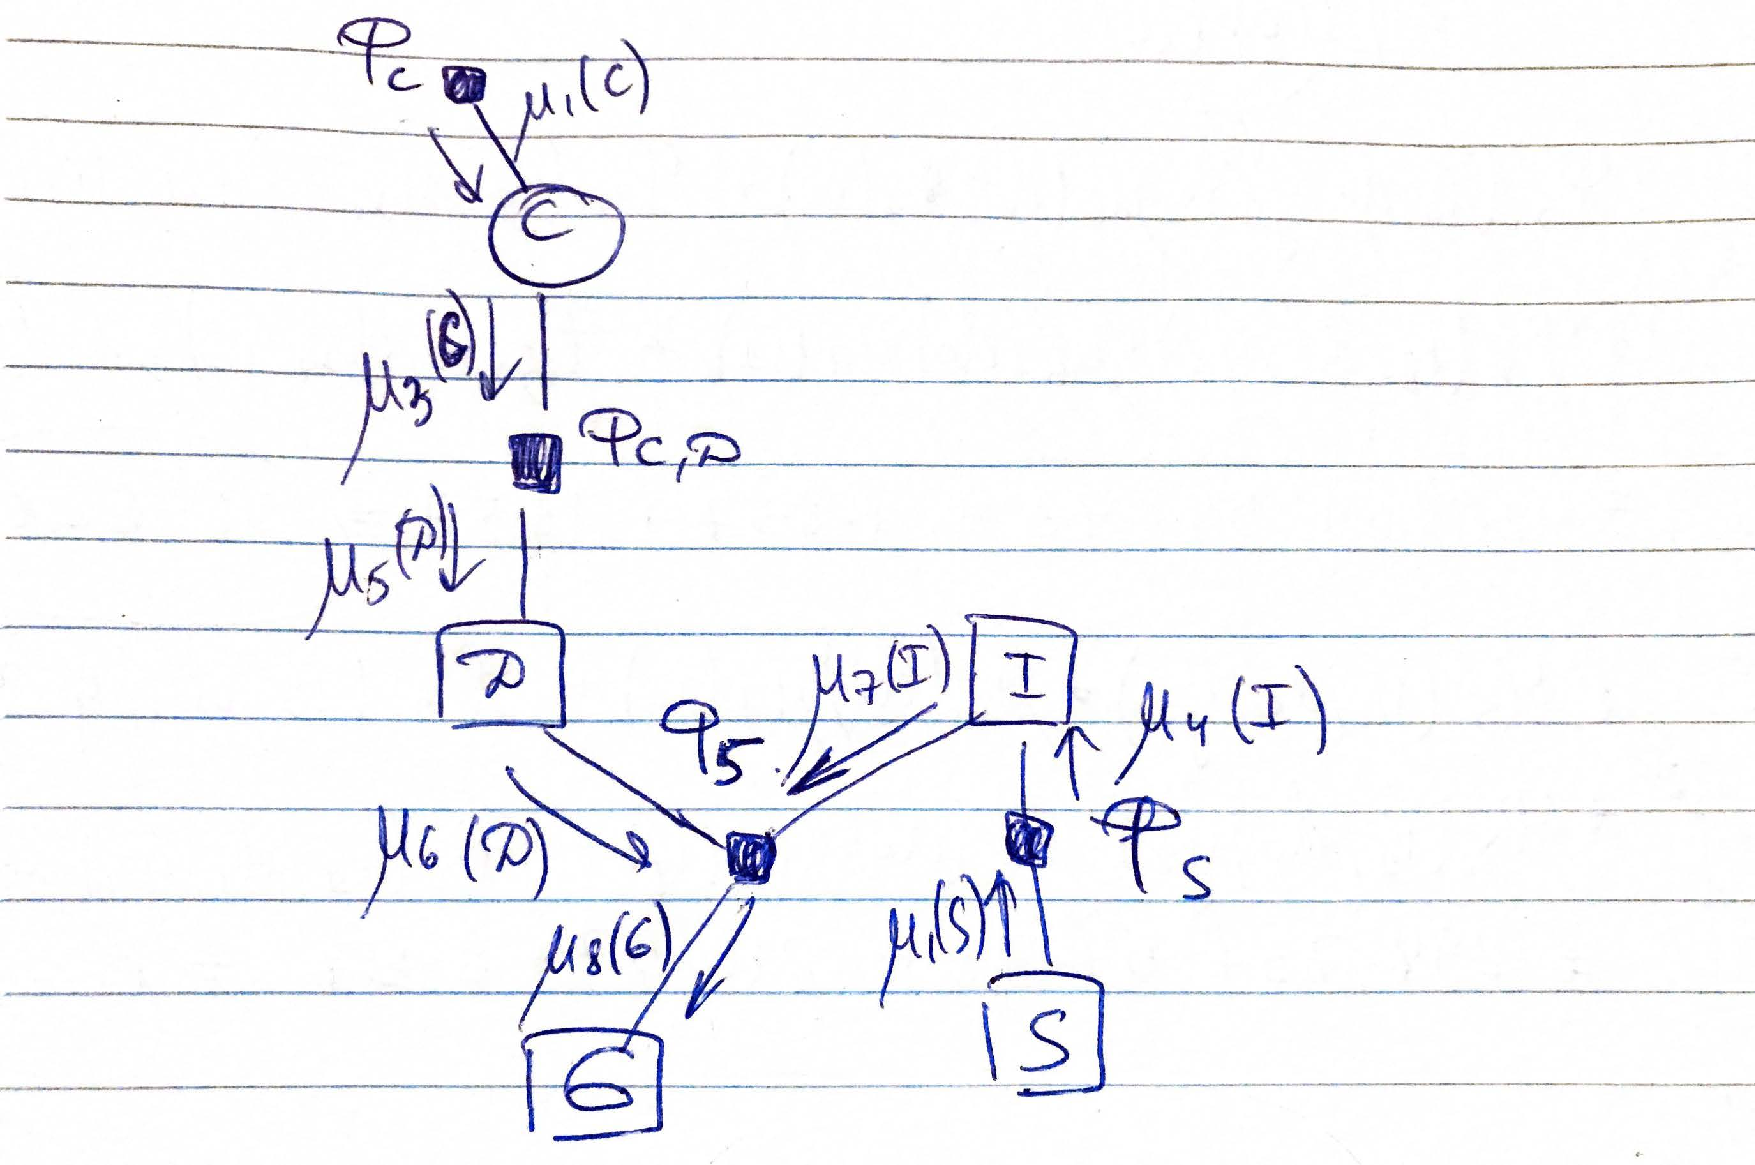
\includegraphics[width = 10cm]{figures/fgraph_3a.pdf}}
	\caption{Factor graph and messages for Exercise 3, Part a}
	\label{fig:fgraph_3a}
\end{figure}

First, we compute the factor $\Phi_5 = \Phi_{D, I} \cdot \Phi_{G, D, I}$ and obtain the following table (Table \ref{tab:f5}) for it:

\begin{table}[H]
	\centering
	\begin{tabular}{l|rrr}
		\toprule
		$\Phi_5$ & $g_0$ & $g_1$ & $g_2$ \\
		\midrule 
		$d_0, i_0$ & 84 & 42 & 294 \\
		$d_0, i_1$ & 72 & 54 & 54 \\
		$d_1, i_0$ & 216 & 108 & 216 \\
		$d_1, i_1$ & 36 & 18 & 6 \\
		\bottomrule
	\end{tabular}
	\caption{Factor $\Phi_5(G, D, I) =  \Phi_{D, I} \cdot \Phi_{G, D, I}$}
	\label{tab:f5}
\end{table}
	
Now we compute the factor $\Phi(G)$ using sum-product algorithm. We view the node $G$ as the root of the factor graph and initiate messages from the leaves. The messages from the leaves are propagated along every link of the network, using the rules of sum-product algorithm described in Bishop 8.4.4, until the root node has receive messages from all other neighbours.

The sequence of messages, propagated through the network, is as follows (you can see them in the Figure \ref{fig:fgraph_3a} as well):
\begin{itemize}
	\item $ \mu_1(C) = [3, 10] $
	\item $ \mu_2(S) = [1, 1] $
	\item $ \mu_3(C) = [3, 10] $
	\item $ \mu_4(I) = [1 \cdot \Phi(s_0, i_0) + 1 \cdot \Phi(s_1, i_0), 1 \cdot \Phi(s_0, i_1) + 1 \cdot \Phi(s_1, i_1)] = [40, 40] $
	\item $ \mu_5(D) = [3 \cdot \Phi(d_0, c_0) + 10 \cdot \Phi(d_0, c_1), 3 \cdot \Phi(d_1, c_0) + 10 \cdot \Phi(d_1, c_1)] = $ \\
	$ = [3 \cdot 1 + 10 \cdot 7, 3 \cdot 9 + 10 \cdot 3] = [73, 57] $
	\item $ \mu_6(D) = [73, 57]$
	\item $ \mu_7(I) = [73 \cdot \Phi(i_0, d_0) + 57 \cdot \Phi(i_0, d_1), 73 \cdot \Phi(i_1, d_0+ 57 \cdot \Phi(i_1, d_1)] = $ \\
	$ = [73 \cdot 14 + 57 \cdot 18, 73 \cdot 6 + 57 \cdot 2] = [2048, 552] $
	\item $ \mu_8(G) = [\sum_{I, D} \Phi_5(I, D, g_0) \cdot \mu_6(D) \cdot \mu_7(I) , \sum_{I, D} \Phi_5(I, D, g_1) \cdot \mu_6(D) \cdot \mu_7(I), \sum_{I, D} \Phi_5(I, D, g_2) \cdot \mu_6(D) \cdot \mu_7(I)] = [84 \cdot 73 \cdot 40 + 72 \cdot 73 \cdot 40 + 216 \cdot 57 \cdot 40 + 36 \cdot 57 \cdot 40, 42 \cdot 73 \cdot 40 + 54 \cdot 73 \cdot 40 + 108 \cdot 57 \cdot 40 + 18 \cdot 57 \cdot 40, 294 \cdot 73 \cdot 40 + 54 \cdot 73 \cdot 40 + 216 \cdot 57 \cdot 40 + 6 \cdot 57 \cdot 40] = [1030080, 567600, 1522320]$
\end{itemize}

	Therefore, $$ \Phi(G) = \mu_8(G) = (1030080, 567600, 1522320). $$
	
	The corresponding probability distribution is then given by:
	$$ P(G) = \left(\frac{1030080}{1030080 + 567600 + 1522320}, \frac{567600}{1030080 + 567600 + 1522320}, \frac{1522320}{1030080 + 567600 + 1522320}\right). $$
	
	$$ P(G) \approx (0.33, 0.18, 0.49). $$
	
	
\subsection*{Part b}
	To compute the conditional factor $\Phi(S \ | \ c_1)$, we introduce one extra factor connecting to the node $C$, which is one for observed value of the variable and zero otherwise: $\Phi_{c_1} = [0, 1]. $
	
	
	The corresponding factor graph and propagated messages which are discussed below are shown on the Figure \ref{fig:fgraph_3b}.
	
	\begin{figure}[H]
		\centering{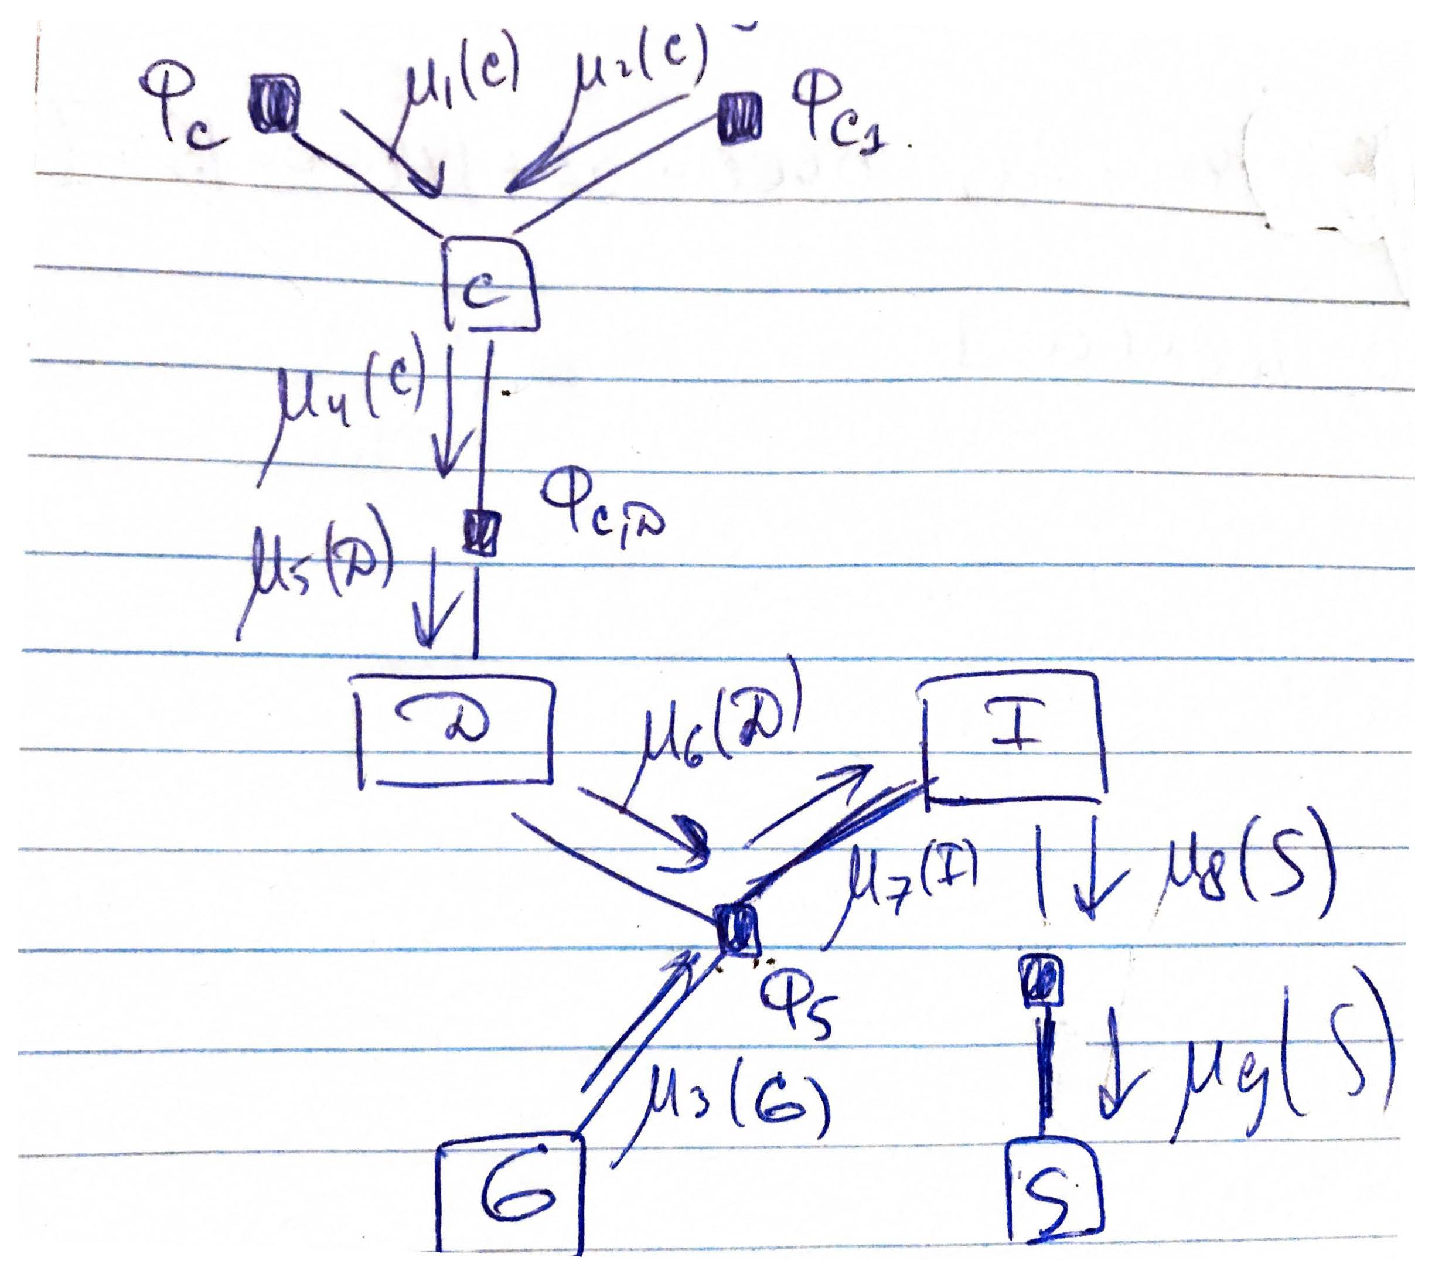
\includegraphics[width = 10cm]{figures/fgraph_3b.pdf}}
		\caption{Factor graph and messages for Exercise 3, Part b}
		\label{fig:fgraph_3b}
	\end{figure}
	
	
	Now we compute the factor $\Phi(S \ | \ c_1)$ using sum-product algorithm. We view the node $S$ as the root of the factor graph and initiate messages from the leaves. The messages from the leaves are propagated along every link of the network, using the rules of sum-product algorithm described in Bishop 8.4.4, until the root node has receive messages from all other neighbours.
	
	The sequence of messages, propagated through the network, is as follows (you can see them in the Figure \ref{fig:fgraph_3b} as well):
	\begin{itemize}
		\item $ \mu_1(C) = [3, 10] $
		\item $ \mu_2(C) = [0, 1] $
		\item $ \mu_3(G) = [1, 1] $
		\item $ \mu_4(C) = [0, 10] $
		\item $ \mu_5(D) = [0 \cdot \Phi(d_0, c_0) + 10 \cdot \Phi(d_0, c_1), 0 \cdot \Phi(d_1, c_0) + 10 \cdot \Phi(d_1, c_1)] = [10 \cdot 7, 10 \cdot 3] = [70, 30] $
		\item $ \mu_6(D) = [70, 30]$
		\item $ \mu_7(I) = \left[\sum_{G, D}\Phi_5 (G, i_0, D) \cdot \mu_3(G) \mu_6(D), \sum_{G, D}\Phi_5 (G, i_1, D) \cdot \mu_3(G) \mu_6(D) \right] = $ \\
		$ = [84 \cdot 1 \cdot 70 + 42 \cdot 1 \cdot 70+ 294 \cdot 1 \cdot 70 + 216 \cdot 1 \cdot 30 + 108 \cdot 1 \cdot 30 + 216 \cdot 1 \cdot 30, 72 \cdot 1 \cdot 70 + 54 \cdot 1 \cdot 70+ 54 \cdot 1 \cdot 70 + 36 \cdot 1 \cdot 30 + 18 \cdot 1 \cdot 30 + 6 \cdot 1 \cdot 30] = [45600, 14400] $
		\item $ \mu_8(I) = \mu_7(I)  = [45600, 14400]$
		\item $ \mu_9(S) = [\mu_8(i_0) \cdot \Phi(i_0, s_0) + \mu_8(i_1) \cdot \Phi(i_1, s_0), \mu_8(i_0) \cdot \Phi(i_0, s_1) + \mu_8(i_1) \cdot \Phi(i_1, s_1)] = [45600 \cdot 8 + 14400 \cdot 24, 45600 \cdot 32 + 14400 \cdot 16] = [710400, 1689600]$
	\end{itemize}
	
	Therefore, $$ \Phi(S | c_1) = (710400, 1689600). $$
	
	
\subsection*{Part c}
	To compute the conditional factor $\Phi(D \ | \ g_2)$, we introduce one extra factor connecting to the node $G$, which is one for observed value of the variable and zero otherwise: $\Phi_{g_2} = [0, 0, 1]. $
	
	
	The corresponding factor graph and propagated messages which are discussed below are shown on the Figure \ref{fig:fgraph_3c}.
	
	\begin{figure}[H]
		\centering{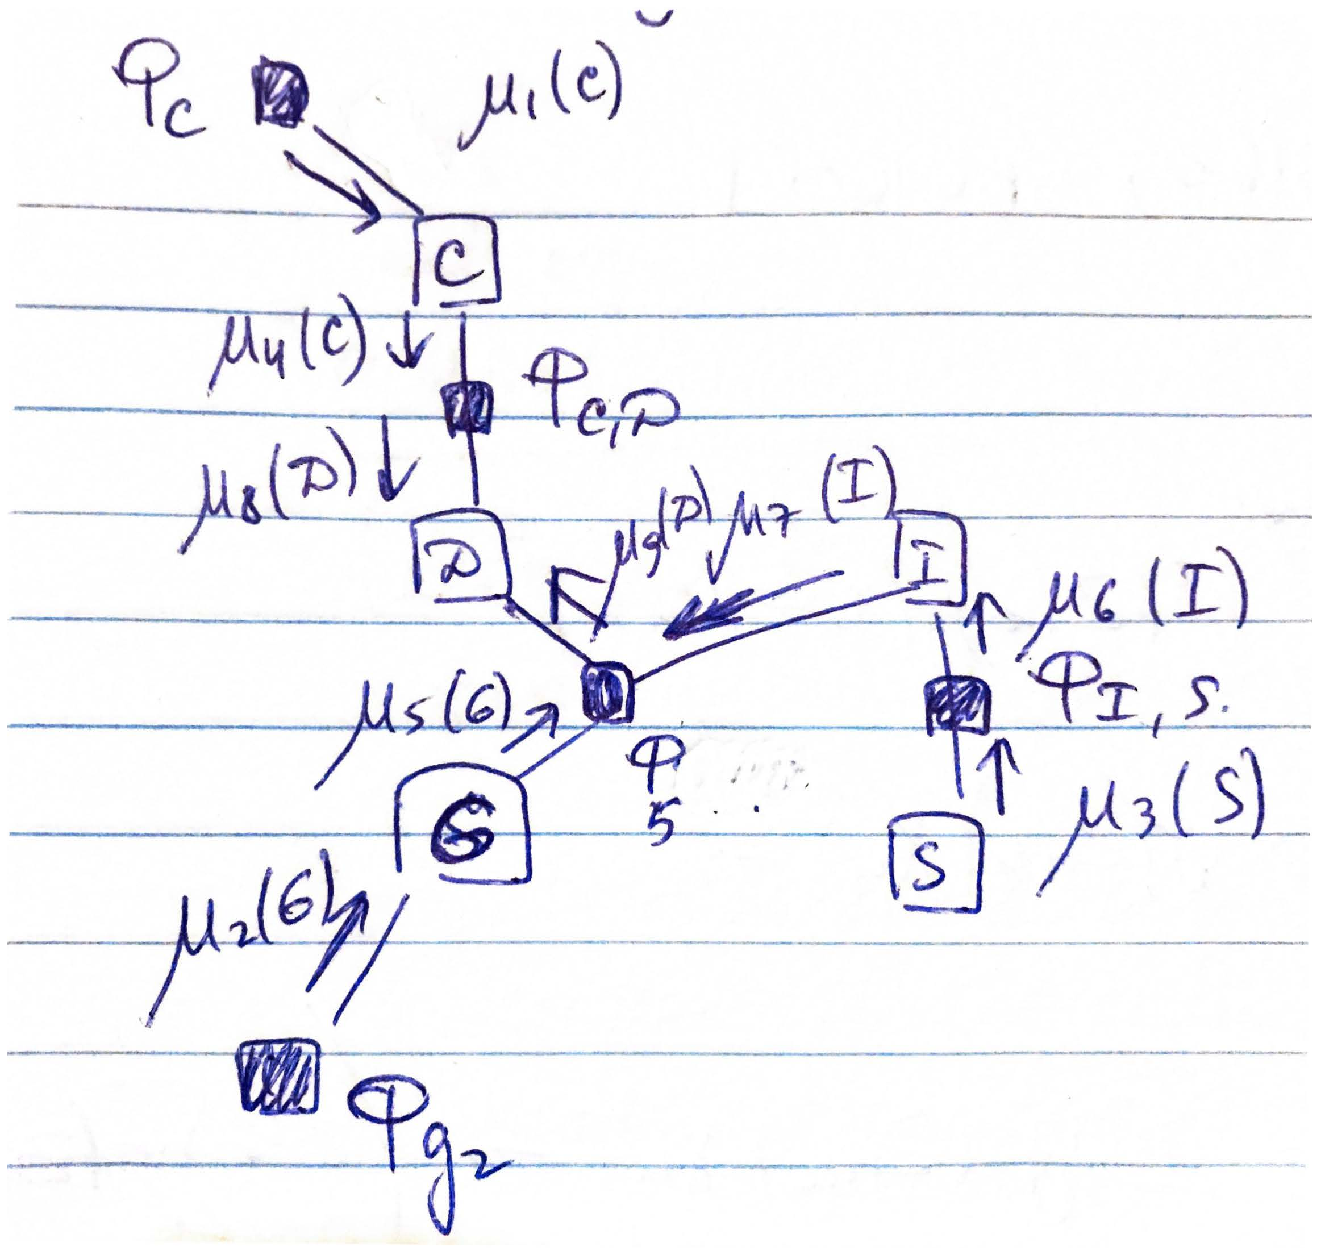
\includegraphics[width = 10cm]{figures/fgraph_3c.pdf}}
		\caption{Factor graph and messages for Exercise 3, Part c}
		\label{fig:fgraph_3c}
	\end{figure}
	
	Now we compute the factor $\Phi(D \ | \ g_2)$ using sum-product algorithm. We view the node $D$ as the root of the factor graph and initiate messages from the leaves. The messages from the leaves are propagated along every link of the network, using the rules of sum-product algorithm described in Bishop 8.4.4, until the root node has receive messages from all other neighbours.
	
	The sequence of messages, propagated through the network, is as follows (you can see them in the Figure \ref{fig:fgraph_3c} as well):
	\begin{itemize}
		\item $ \mu_1(C) = [3, 10] $
		\item $ \mu_2(G) = [0, 0, 1] $
		\item $ \mu_3(S) = [1, 1] $
		\item $ \mu_4(C) = [3, 10] $
		\item $ \mu_5(G) = [0, 0, 1]$
		\item $ \mu_6(I) = [\Phi(i_0, s_0) \cdot \mu_3(s_0) +  \Phi(i_0, s_1) \cdot \mu_3(s_1), \Phi(i_1, s_0) \cdot \mu_3(s_0) +  \Phi(i_1, s_1) \cdot \mu_3(s_1)] = $\\ $ = [8 \cdot 1 + 32 \cdot 1, 24 \cdot 1 + 16 \cdot 1] = [40, 40]$ 
		\item $ \mu_7(I) = \mu_6(I) = [40, 40]$
		\item $ \mu_8(D) = [\Phi(d_0, c_0) \mu_4(c_0) +  \Phi(d_0, c_1) \mu_4(c_1), \Phi(d_1, c_0) \mu_4(c_0) +  \Phi(d_1, c_1) \mu_4(c_1)] = $ \\
		$ [1 \cdot 3 + 7 \cdot 10, 9 \cdot 3 + 3 \cdot 10] = [73, 57]$
		\item $ \mu_9(D) = \left[\sum_{G, I}\Phi_5(G, I, d_0) \cdot \mu_5(G) \mu_7(I),  \sum_{G, I}\Phi_5(G, I, d_1) \cdot \mu_5(G) \mu_7(I) \right] = [13920, 8880].$
		
	\end{itemize}
	
	$$ \Phi(D, g_2) = \mu_8(D) \cdot \mu_9(D) = [13920 \cdot 73, 8880 \cdot 57] = [1016160, 506160] $$
	
	The corresponding probability distribution, $P(D | g_2)$ is given by:
	$$ P(D | g_2) = \left(\frac{\Phi(d_0 | g_2)}{\sum_{D}\Phi(D | g_2)}, \frac{\Phi(d_1 | g_2)}{\sum_{D}\Phi(D | g_2)}\right) = \left(\frac{1016160}{1016160+506160},\frac{506160}{1016160+506160}\right) $$
	
	So,
	$$ P(D | g_2) \approx (0.67,0.33) $$
	
	
	
	
\end{document}